\documentclass[a0,landscape]{a0poster}

\usepackage{multicol}
\columnsep=100pt
\columnseprule=3pt

\usepackage[svgnames]{xcolor}

\usepackage[scaled]{helvet}
\renewcommand\familydefault{\sfdefault}
\usepackage[T1]{fontenc}

\usepackage{float}
\usepackage{tikz}
\usetikzlibrary{patterns}
\usetikzlibrary{trees}
\usetikzlibrary{shapes}
\usetikzlibrary{calc}

\usepackage{graphicx}
\graphicspath{{figures/}}
\usepackage{booktabs}
\usepackage[font=small,labelfont=bf]{caption}
\usepackage{amsfonts, amsmath, amsthm, amssymb}
\usepackage{wrapfig}
\usepackage{subcaption}


\begin{document}

\begin{minipage}[b]{0.7\linewidth}
\veryHuge \color{NavyBlue} \textbf{Building Game Theoretical Software in a Research Environment} \color{Black}\\ % Title
\Huge\textit{With an application to healthcare modelling}\\[1cm] % Subtitle
\huge \textbf{James Campbell \& Dr Vince(nt) Knight}\\ % Author(s)
\huge School of Mathematics\\ % University/organization
\end{minipage}
%
%
\begin{minipage}[b]{0.3\linewidth}
\centering

\includegraphics[width=15cm]{Images/logo.eps}
\end{minipage}

\vspace{1cm}
\begin{multicols}{3}


\begin{figure}[H]
\centering

\includegraphics[width=0.9\linewidth]{Images/sage-banner-02.png}
\end{figure}

\color{Brown}
\section*{Sage open-source mathematical software system}
Sage: "Creating a viable free open source alternative to Magma, Maple, Mathematica and Matlab".
Ref?
Sage is Open Source, which means that anyone can contribute to it's upkeep and improvement, but only after a stringent review scheme.
We settled on three projects to add to Sage, one of which has already been included in a recent release.

\section*{Our Contribution}
\begin{itemize}
    \item Normal Form Games;
    \item Matching Games;
    \item Cooperative Games.
\end{itemize}

Matching Games allow us to solve problems where players need to be paired with each other, but they have their own preferences.
We normally look for stable matching where no player has any incentive to change their pairing.

\begin{figure}[H]
\color{Black}
\centering
\tikzstyle{level 1}=[level distance=3.5cm, sibling distance=3.5cm]
\tikzstyle{level 2}=[level distance=3.5cm, sibling distance=2cm]
\tikzstyle{level 3}=[level distance=3.5cm, sibling distance=1cm]
\tikzstyle{player} = [text width=5em, draw, text centered, rectangle, fill=blue!20, inner sep=1pt]
\tikzstyle{nature} = [minimum width=3pt,circle,  draw, fill=red!20, inner sep=1pt]
\tikzstyle{end} = [circle, minimum width=3pt, fill, inner sep=0pt, right]
\begin{tikzpicture}
    \node (a) [end] at (0,0) {};
    \node (b) [end] at (0,1) {};
    \node (c) [end] at (0,2) {};
    \node (A) [end] at (2,0) {};
    \node (B) [end] at (2,1) {};
    \node (C) [end] at (2,2) {};
    \node [left] at (a) {$a$: $(A,B,C)$};
    \node [left] at (b) {$b$: $(B,C,A)$};
    \node [left] at (c) {$c$: $(B,A,C)$};
    \node [right] at (A) {$A$: $(b,c,a)$};
    \node [right] at (B) {$B$: $(a,c,b)$};
    \node [right] at (C) {$C$: $(a,b,c)$};
    \draw (c) -- (A);
    \draw (a) -- (B);
    \draw (b) -- (C);
\end{tikzpicture}
\caption{A stable matching}
\label{fig:matching_game}
\end{figure}

Co-operative Games are used in situations where players each contribute to a system and those separate contributions require their own payoff.
Normal Form Games involve players choosing different strategies against each other and obtaining a payoff.
Nash equilibria occur when no player has any incentive to change which strategy they play.

\color{Goldenrod}
\section*{Stackelberg game}
The issue of waiting times for ambulances at at two hospitals can be modelled as a 3 player Stackelberg game where each hospital has its own AE and Ward.


{\color{black}
\begin{figure}[H]
    \begin{center}
        \tikzstyle{level 1}=[level distance=8.5cm, sibling distance=6.5cm]
        \tikzstyle{level 2}=[level distance=8.5cm, sibling distance=4cm]
        \tikzstyle{player} = [draw, text centered, rectangle, fill=blue!20, inner sep=1pt]
        \tikzstyle{nature} = [minimum width=3pt,circle,  draw, fill=red!20, inner sep=1pt]
        \tikzstyle{end} = [circle, minimum width=3pt, fill, inner sep=0pt, right]
        \tikzstyle{corner} = [inner sep=0pt, outer sep=0pt, draw,circle]
        \begin{tikzpicture}[grow=right, sloped, scale=.6]
            \node[player]{H1}
            child {node [corner] (A1) {} node [right=2pt]{$C^{(1)} - 1$} }
            child {node [corner] (A2) {} node [right=2pt] {$1$} edge from parent node[above] {$\color{blue}{c^{(1)}}$}} ;
            \draw [bend right, dashed] (A1) to (A2);
            \node (B3) [player,right=3pt] at ($(A1)!0.5!(A2)$) {H2}
            child {node [corner] (A3) {} node [right=2pt]{$C^{(2)} - 1$} }
            child {node [corner] (A4) {} node [right=2pt] {$1$} edge from parent node[above] {$\color{red}{c^{(2)}}$}} ;
            \draw [bend right] (A3) to (A4);
            \node (e) [player,right=3pt] at ($(A3)!0.5!(A4)$) {A}
            child {node [corner] (A5) {} node [right=2pt]{$\Lambda$} }
            child {node [corner] (A6) {}  node [right=2pt] {$0$}edge from parent node[above] {$\lambda_1$}} ;
            \draw [bend right] (A5) to (A6);
            \node (e) [end,right=7pt] at ($(A5)!0.5!(A6)$) {};
        \end{tikzpicture}
        \caption{Underlying Stackelberg Game}\label{fig:stackelberg_game}
    \end{center}
\end{figure}
}

Patients arrive at the AE at rate $\lambda$ and if there is space in the queue they join it.
If there is no space in the queue that patient is lost.
Each patient has an AE service time, $\mu$, which represents how long their treatment in AE will last.
A proportion, $p$, of patients are then dismissed immediately.
Those who are not dismissed are admitted to the ward if there is space, otherwise they will wait in AE, continuing to occupy a bed.
Once admitted, they are treated in the ward with a service time $\hat{\mu}$ and then dismissed without delay.

\begin{figure}[H]
\centering
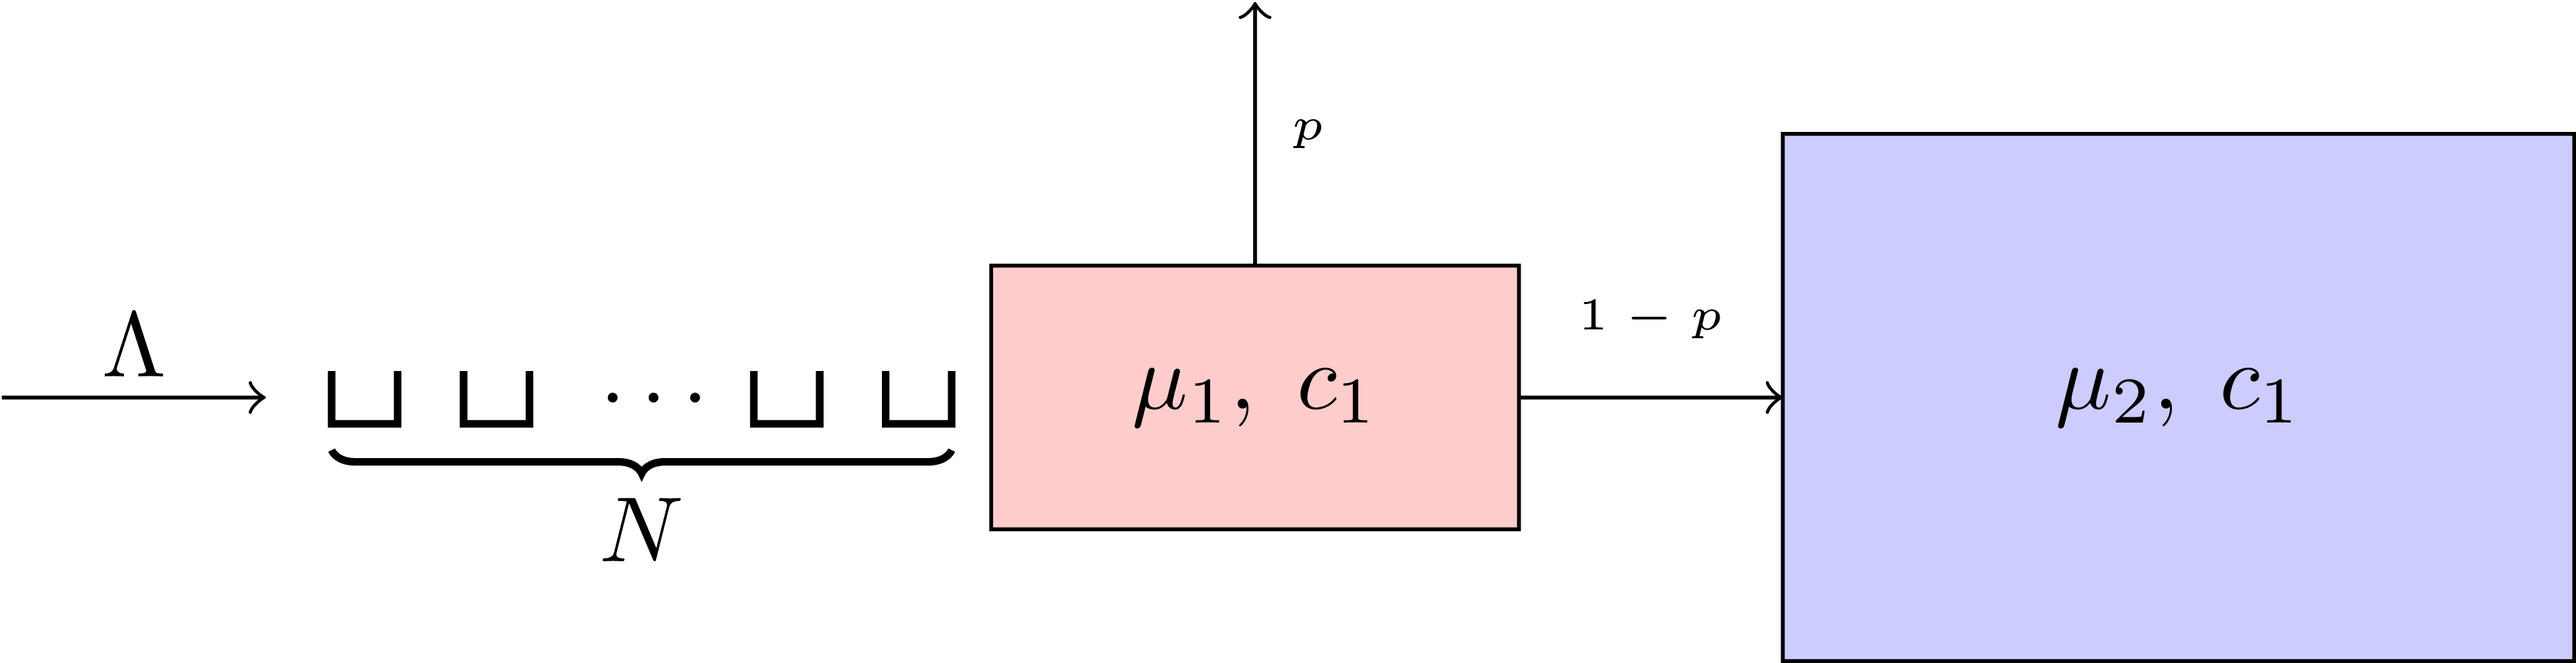
\includegraphics[width=0.9\linewidth]{Images/tandem_queue.png}
\caption{The system}
\label{fig:tandem_queue}
\end{figure}

\section*{Markov Chain}
A Markov Chain is ideal for this because the system is memoryless, ie. at any one time the probability of a patient arriving or finishing their service is independent of what has happened before.

\begin{figure}[H]
\centering
\includegraphics[width=0.9\linewidth]{Images/{12-11-12-1.0-0.2-0.7}.pdf}
\caption{Theoretical and simulated expected wait times}
\label{fig:wait_times}
\end{figure}

\color{Olive}
\section*{Validation}
One of our most important jobs was to validate the Markov Chain that we had created.
This was achieved by comparing various results from a Monte Carlo simulation with analytical results from the Markov Chain.\\
\\
One way of doing this was to compare the Mean Expected wait for different arrival rate $\lambda$.
In fig \ref{fig:wait_times} the blue is our analytical approach and the box plots show simulated data that we recorded.\\
\\
Fig \ref{fig:markov_chain_example_pdf_2} shows the probability of being in state $(i,j)$ for varying $\lambda$.
Again it compares analytical results to simulated ones.


\section*{Limitations of MC}
The main problem with the Markov Chain approach is that calculating the payoffs required for the associated Normal Form Game is very CPU intensive.
It therefore required use of the Cardiff Univeristy supercomputer, RAVEN.
If the Normal Form Games themselves became too large, solving them to obatin Nash Equilibria could also take a significant amount of time.\\
\\
It also assumes that the ambulances do not observe the system.


\color{SteelBlue}
\section*{Markov Decision Process}
A Markov Decision Process is a model of decision making in a dynamic framework in which a decision maker makes decisions based on a particular system state \cite{puterman2009markov}.
The process is that an agent starts off in a particular state, makes a decision, and then has a probabilistic transition whose probabilities may depend on the previous decision.

\section*{Q-Learning}
Q-learning is the process of assigning a state-action value or Q-value to the combination of being in a state, taking an action and observing a reward.
The Q-value is then updated by assessing the maximum value of being in the new state.
The higher the Q-value the more likely a player is to choose action $a$ when in state $s$.


\begin{figure}[H]
    \centering
        \begin{subfigure}{.4\linewidth}
            \includegraphics[width=\textwidth]{./Images/{10.000-15.000-12.000-4.000-0.400-1.000-0.200-40000.000-10000.000-32-markov_chain}.pdf}
        \caption{Markov Chain for $\Lambda=4$}\label{fig:markov_chain_example_pdf_mc_4}
        \end{subfigure}
        \begin{subfigure}{.4\linewidth}
            \includegraphics[width=\textwidth]{./Images/{10.000-15.000-12.000-4.000-0.400-1.000-0.200-40000.000-10000.000-32-simulation}.pdf}
        \caption{Simulation for $\Lambda=4$}\label{fig:markov_chain_example_pdf_sim_4}
        \end{subfigure}
        \\
        \begin{subfigure}{.4\linewidth}
            \includegraphics[width=\textwidth]{./Images/{10.000-15.000-12.000-4.500-0.400-1.000-0.200-40000.000-10000.000-32-markov_chain}.pdf}
        \caption{Markov Chain for $\Lambda=4.5$}\label{fig:markov_chain_example_pdf_mc_4.5}
        \end{subfigure}
        \begin{subfigure}{.4\linewidth}
            \includegraphics[width=\textwidth]{./Images/{10.000-15.000-12.000-4.500-0.400-1.000-0.200-40000.000-10000.000-32-simulation}.pdf}
        \caption{Simulation for $\Lambda=4.5$}\label{fig:markov_chain_example_pdf_sim_4.5}
        \end{subfigure}
        \\
        \begin{subfigure}{.4\linewidth}
            \includegraphics[width=\textwidth]{./Images/{10.000-15.000-12.000-5.000-0.400-1.000-0.200-40000.000-10000.000-32-markov_chain}.pdf}
        \caption{Markov Chain for $\Lambda=5$}\label{fig:markov_chain_example_pdf_mc_5}
        \end{subfigure}
        \begin{subfigure}{.4\linewidth}
            \includegraphics[width=\textwidth]{./Images/{10.000-15.000-12.000-5.000-0.400-1.000-0.200-40000.000-10000.000-32-simulation}.pdf}
        \caption{Simulation for $\Lambda=5$}\label{fig:markov_chain_example_pdf_sim_5}
        \end{subfigure}
        \\
    \caption{Theoretical and simulated distribution of $\pi$ for $\Lambda\in\{4,4.5,5\}$}
    \label{fig:markov_chain_example_pdf_2}
\end{figure}

\end{multicols}
\end{document}
